\documentclass[english, twocolumn, 10pt, aps, superscriptaddress, floatfix, prb, citeautoscript]{revtex4-1}
\pdfoutput=1
\usepackage[utf8]{inputenc}
\usepackage[T1]{fontenc}
\usepackage{verbatim}
\usepackage{units}
\usepackage{mathtools}
\usepackage{amsmath}
\usepackage{amssymb}
\usepackage{graphicx}
\usepackage{wasysym}
\usepackage{layouts}
\usepackage{siunitx}
\usepackage{bm}
\usepackage{xcolor}
\usepackage[colorlinks, citecolor={blue!50!black}, urlcolor={blue!50!black}, linkcolor={red!50!black}]{hyperref}
\usepackage{bookmark}
\usepackage{tabularx}
\usepackage{microtype}
\usepackage{babel}
\hypersetup{pdfauthor={Quantum Tinkerer},pdftitle={Enhanced proximity effect in zigzag-shaped Majorana Josephson junctions.}}

\setcounter{secnumdepth}{4}
\setcounter{tocdepth}{4}

\DeclareMathOperator{\e}{e}
\DeclareMathOperator{\de}{d\!}
\DeclareMathOperator{\Tr}{Tr}
\DeclareMathOperator{\diag}{diag}
\DeclareMathOperator{\Res}{Res}
\DeclareMathOperator{\sgn}{sgn}
\DeclareMathOperator{\Pf}{Pf}
\DeclareMathOperator{\Det}{Det}
\DeclareMathOperator{\rank}{rank}
\DeclareMathOperator{\im}{Im}
\DeclareMathOperator{\re}{Re}
\newcommand{\kx}{k_x}
\newcommand{\ky}{k_y}
\newcommand{\meff}{m_\text{eff}}

\renewcommand{\comment}[2]{#2}
% Uncomment the following line for paragraph descriptions to appear in the file.
\renewcommand{\comment}{\paragraph}

\DeclarePairedDelimiter\abs{\lvert}{\rvert}
\DeclarePairedDelimiter\norm{\lVert}{\rVert}

\makeatletter
\let\oldabs\abs
\def\abs{\@ifstar{\oldabs}{\oldabs*}}
\let\oldnorm\norm
\def\norm{\@ifstar{\oldnorm}{\oldnorm*}}
\makeatother

\newcommand{\ev}[1]{\langle#1\rangle}
\newcommand{\bra}[1]{\langle#1|}
\newcommand{\ket}[1]{|#1\rangle}
\newcommand{\bracket}[2]{\langle#1|#2\rangle}

\newcolumntype{L}[1]{>{\raggedright\arraybackslash}p{#1}}
\newcolumntype{C}[1]{>{\centering\arraybackslash}p{#1}}
\newcolumntype{R}[1]{>{\raggedleft\arraybackslash}p{#1}}


\begin{document}


\title{Enhanced proximity effect in zigzag-shaped Majorana Josephson junctions.}

\author{Quantum Tinkerer}
\affiliation{Kavli Institute of Nanoscience, Delft University of Technology, P.O. Box 4056, 2600 GA Delft, The Netherlands}
\email[Electronic address: ]{quantumtinkerer@tudelft.nl}

\date{\today}
\begin{abstract}
High density superconductor-semiconductor-superconductor junctions have a small induced superconducting gap due to the quasiparticle trajectories with a large momentum parallel to the junction, because these trajectories have a very long flight time.
Because a large induced gap protects Majorana modes, these long trajectories constrain Majorana devices to low electron density.
We show that a zigzag-shaped geometry eliminates these trajectories, allowing the robust creation of Majorana states with both the induced gap and the Majorana size improved by more than an order of magnitude for realistic parameters.
In addition to the improved robustness of Majoranas, this new zigzag geometry is insensitive to the geometric details and the device tuning.
\end{abstract}

\maketitle

%%██████████████████████████████████████████████████████████████████████████
%%██ Introduction
%%██████████████████████████████████████████████████████████████████████████
\section{Introduction}
\comment{Hybrid NS structures become topological and are useful for TQC.}
A hybrid structure containing a semiconductor with strong spin-orbit coupling coupled to a superconductor, inside a magnetic field becomes topological within the right parameter regime ($E_z^2>\mu^2+\Delta^2$ for a simple nanowire), while Majorana bound states appear on its edges.~\cite{lutchyn_majorana_2010,oreg_helical_2010}
Majorana bound states are a promising candidate to form the basis of a stable platform for topological quantum computing. ~\cite{alicea2012new,beenakker2013search}
The current experimental effort ~\cite{mourik_signatures_2012,das_zero-bias_2012,deng_anomalous_2012,churchill_superconductor-nanowire_2013,zhang2018quantized} focuses on creating pairs of Majorana bound states in hybrid normal-superconductor (NS) nanowires structures.

\comment{The gap is small because of long trajectories.}
One of the biggest challenges in creating stable Majoranas is the appearance of a soft gap~\cite{ren_topological_2018}; where the gap in the density of states significantly reduces for states with the momentum directed along the length of the strip.
From a semiclassical perspective, these momenta correspond to long paths through the semiconductor without interruption by the superconductor.
Additionally, these long trajectories have long flight times $\tau_f \approx D / v_F$ (see Fig.~\ref{fig:setup}), with $D$ the trajectory length.
Equivalently, the Thouless energies $E_{\textrm{Th}}=\hbar / \tau_f$ are small, resulting in a small gap.
This problem does not appear when the Fermi surface is small and the zero point motion dominates the transverse velocity, so a low filling of the bands is a workaround\cite{nijholt2015orbital}.
However, low filling requires precise knowledge of the system and might be more sensitive to disorder or microscopic inhomogeneities.
On the other hand, disorder scatters these long trajectories and introduces a cut-off on the scale of the mean-free path~\cite{haim_double-edge_2018}, however, disorder is impossible to control to a required precision experimentally.

\begin{figure}[!htb]
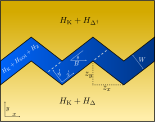
\includegraphics[width=\columnwidth]{figures/zigzag.pdf}
\caption{Setup of the straight (top) and the zigzag (bottom) SNS junction.
The yellow areas are the superconductors at a phase difference $\pm \phi / 2$.
The middle area is the semiconductor of width $W$ and has a magnetic field $B$ in the $x$-direction.
The modulation of the zigzag is parameterized by its amplitude $z_y$ and period $z_x$.
Inside the semiconductor we indicate the longest possible trajectory by the red curve.
\label{fig:setup}}
\end{figure}

\comment{A alternative has been proposed.}
Recently, a system with a modification has been proposed\cite{pientka2017topological}, where instead of having one superconductor, there are two superconductors, creating a superconductors-normal-superconductor (SNS) junction.
The additional superconductor adds an extra knob to adjust, the superconducting phase difference $\phi$, and this should make it easier to tune the system into the topological phase.
Recently, two groups~\cite{fornieri_evidence_2018,ren_topological_2018} have realized this system experimentally.
In practice, multiple problems arise making even the observation difficult, rendering the manipulation of Majoranas in the near future, improbable.

\comment{We show that zigzag geometry solves this problem by eliminating the long trajectories.}
We propose a new experimental setup (see Fig.~\ref{fig:setup}(b)) for the creation of Majoranas that eliminating long trajectories and therefore prevents the appearance of a soft gap, while while also increasing the topological gap by several orders of magnitude, depending on the parameters.
The setup consists of a zigzag or snake-like geometry for the semiconductor where long trajectories are not possible due to the geometry.
In this paper we will focus on two-dimensional (2D) Josephson junctions, however, a zigzag geometry will also work for nanowires.\footnote{We confirmed this numerically, although it is not included in this paper.}


%%██████████████████████████████████████████████████████████████████████████
%%██ Setup
%%██████████████████████████████████████████████████████████████████████████
\section{Setup}\label{sec:setup}

\comment{We consider a two-dimensional system with zigzag and BdG Hamiltonian.}
We consider a Josephson junction (Fig.~\ref{fig:setup}) consisting of a 2D strip of semiconductor, with superconductors on both sides.
We modulate the shape of the normal region, which can be either saw-toothed zigzag as depicted [Fig.~\ref{fig:setup}(b)], or a more smooth sinusoidal-like shape.
Similar to the conventional straight system \cite{pientka2017topological}, a magnetic field $B_x$ perpendicular to the junction is applied.
We model the system with a Bogoliubov-de Gennes Hamiltonian (BdG) Eq.~\eqref{eq:hamiltonian}; the normal part has a linear Rashba spin-orbit coupling term characterized by $\alpha$ and a Zeeman field with $E_z=\frac{1}{2} \mu_B g B_x$.
The superconductor has a superconducting coupling term $\Delta$ with the pair of superconductors at an opposite superconducting phase $\exp{\pm i \phi/2}$.
Both the normal part and the superconducters have a kinetic term and chemical potential $\mu$.
The complete Hamiltonian has the form
\begin{subequations}
\begin{align}
    H_\textrm{N} = & \left[\frac{\hbar^2\left(\kx^2 + \ky^2\right)}{2\meff} - \mu + \alpha \left( \ky \sigma_x - \kx \sigma_y \right) \right] \tau_z
        + E_\text{z} \sigma_x \\
    H_\textrm{SC} = & \left[\frac{\hbar^2\left(\kx^2 + \ky^2\right)}{2\meff} - \mu\right] \tau_z
        + \Delta \cos{\frac{\phi}{2}} \tau_x + \Delta \sin{\frac{\phi}{2}} \tau_y.
\end{align}
\label{eq:hamiltonian}
\end{subequations}
Where $H_\textrm{N}$ and $H_\textrm{SC}$ are the Hamiltonians of the semiconductor and superconductors, respectively.
They act on the spinor wave function $\Psi={\left(\psi_{e\uparrow},\psi_{e\downarrow},\psi_{\textrm{h}\downarrow},-\psi_{\textrm{h}\uparrow}\right)}^{T}$, where $\psi_e$, $\psi_\textrm{h}$ are its electron and hole components, and $\psi_\uparrow$, $\psi_\downarrow$ are the spin-up and spin-down components.
The Pauli matrices $\sigma_{i}$ act on the spin degree of freedom and $\tau_{i}$ act on the electron-hole degree of freedom.
For the zigzag geometry, we first consider a sawtooth-like pattern where $z_x$ is periodicity, $z_y$ the amplitude and $W$ the width of the junction [see Fig.~\ref{fig:setup}(b)].
Later in this manuscript, we show that the exact details of the shape are unimportant and consider different zigzag geometries also parametrized by $z_x, \; z_y, \; W$.

\comment{We discretize the Hamiltonian and simulate it with Kwant.}
We discretize our continuum Hamiltonian [Eq.~\eqref{eq:hamiltonian}] on a square grid and implement a tight-binding model using Kwant~\cite{groth_kwant:_2014}.
To preferentially sample important regions of parameter space, we use the Adaptive package.~\cite{adaptive}
The entire source code and the resulting raw data are available in Ref.~\onlinecite{data}.  % TODO: update the bib when the data is uploaded

\comment{The default parameters are ...}
Unless noted differently, the Hamiltonian parameters are $\alpha=\SI{20}{\meV \nm}$, $g=26$, $\meff=\SI{0.02}{\electronmass}$, $\mu=\SI{10}{\meV}$, $B=\SI{1}{T}$, $\phi=\pi$, and $\Delta=\SI{1}{\meV}$; and the geometry parameters are $W=\SI{200}{\nm}$, the period of the zigzag $z_x=\SI{1300}{\nm}$, the discretization contant $a=\SI{10}{\nm}$, and the lengths of the superconductors $L_\textrm{SC}=\SI{300}{\nm}$.  % TODO: Tom: L_sc and Delta not compatible?


%%██████████████████████████████████████████████████████████████████████████
%%██ Band stuctures
%%██████████████████████████████████████████████████████████████████████████
\section{Band stuctures}\label{sec:band_structures}

\begin{figure}[!htb]
\includegraphics[width=\columnwidth]{figures/bandstructures}
\caption{Figure of the band stuctures corresponding to the system in Fig.~\ref{fig:setup} with different zigzag amplitudes.
The blue lines correspond to $\phi=0$, $B=0$ (trivial phase) and the orange lines to $\phi=\pi$, $B = \SI{1}{T}$ (topological phase).
The three subplots are for different amplitudes of the zigzag, with (a) a straight system $z_y=0$, (b) $z_y=\frac{W}{2}$, and (c) $z_y=W$, where $W=\SI{200}{\nm}$ is the junction width.
On the $x$-axis is the folded lattice momentum where $z_x=\SI{1300}{\nm}$.
Subplot (a) has a different scale on the $x$-axis for $k_x < 0$ than the other subplots and displays the unfolded band structure.
For the right-hand side of (a) ($k_x > 0$), (b), and (c), the folding is the same, such that the velocity $v=\frac{dE}{dk}$ can be compared visually.
We observe that once there are no more straight trajectories inside the junction (when $z_y=W$) the spectrum becomes most insensitive to the momentum $k_x$, and thus the $v_\textrm{F}$ decreases.
As the zigzag amplitude increases the band gap $E_\textrm{gap}$ increases by an order of magnitude.
The combination of these ensures a significant decrease of the Majorana decay length because $\xi_M \propto \frac{v_\textrm{F}}{E_\textrm{gap}}$
The parameters values are written at the end of Sec.~\ref{sec:setup}.\label{fig:band_structures}}
% TODO: mention z_x!
\end{figure}

\comment{We calculate the band structure for varying amount of zigzag.}
We apply sparse diagonalization to the supercell Hamiltonian at different momenta $k_x$ to compute the band structure.
Because of the large periodicity of the zigzag and the resulting large supercell, the band structure is heavily folded.
In figure~\ref{fig:band_structures} we show the resulting band structures for zigzag systems with a varying amplitude.
The introduction of the zigzag has a striking effect: the bands flatten out and the topological gap increases by more than an order of magnitude.

\comment{Zigzag improves the gap and size because of cutting of trajectories and increasing transparency.}
This confirms our expectation that the zigzag removes trajectories propagating at grazing angles.
In the unfolded band structure for a straight system, as seen in Fig.~\ref{fig:band_structures}(a), the gap in a straight system occurs around $k_F$ and because the zigzag cuts off long trajectories, the gap size increases.
Besides this, the states from different segments of the zigzag pattern have a negligible overlap and therefore have a vanishing velocity.
This reduction in velocity strongly reduces the Majorana size, as we discuss in section \ref{sec:shape_effects}.
Additionally, in the presence of normal reflection, due to the presence of NS interfaces at a wide range of angles, the reflected part eventually scatters with a near perpendicular surface.
This means that for transversal modes the transparency of the NS interface increases.

%%██████████████████████████████████████████████████████████████████████████
%%██ Localization lengths and shape effect
%%██████████████████████████████████████████████████████████████████████████
\section{Localization lengths and shape effects}\label{sec:shape_effects}

\begin{figure}[!htb]
\includegraphics[width=\columnwidth]{figures/wavefunctions}
\caption{Density of wavefunctions $\left|\psi\right|^2$ for sizes and geometries.
With (a) a straight system, (b) a saw-toothed zigzag system, (c) a system where the normal region is defined by lines parallel to a sinusoid, and (d) similar to (c) but with disordered edges.
Inside the figure, we indicate the Majorana length (or coherence length) $\xi_\textrm{M}$, the Majorana energy $E_\textrm{M}$ (the energy of the first excited state), and the topological energy gap $E_\textrm{gap}$.
We observe that $\xi_\textrm{M}$ for (a) is almost two orders of magnitude longer and $E_\textrm{gap}$ more than an order of magnitude smaller than for (b), (c), and (d).
The robustness of $E_\textrm{gap}$ and $\xi_\textrm{M}$ across (b), (c), and (d) means that the details of the geometry do not matter for the improvements to occur.
The length of the system is $3.5 L_x=\SI{4550}{\nm}$, the remaining parameters values are written at the end of Sec.~\ref{sec:setup}.\label{fig:wavefunctions}}
\end{figure}

\comment{We calculate the wave functions and find the Majorana lengths by fitting an exponential.}
We model a finite system to compute the Majorana wave function density for different geometries; ribbon, saw-toothed zigzag, parallel curves, and variants of the latter with disordered edges.
By diagonalizing the Hamiltonian, we find the Majorana energy $E_\textrm{M}$ and the energy of the first excited state $E_1$, the lowest and second lowest energies, respectively.
Using the eigenstates, we calculate the Majorana decay length $\xi_\textrm{M}$ by fitting an exponential to the density of a single Majorana wavefunction projected on the $x$-axis.
To determine $\xi_\textrm{M}$, we use a trick and artificially break the particle-hole symmetry on one edge by adding a potential $V \sigma_0 \tau_0$ such that one of the Majorana states is pushed into the continuum and the fit to $\exp{\frac{x}{\xi_\textrm{M}}}$ becomes easier.
In figure~\ref{fig:wavefunctions} the wavefunctions are displayed, superimposed upon their respective geometry.
All systems have identical Hamiltonian parameters in order to compare the effects of the changing geometry meaningfully.

\comment{In a straight system, the Majoranas are very poorly localized.}
For the ribbon system [Fig.~\ref{fig:wavefunctions}(a)], we see that the decay of the density is long compared to the system size.
The wavefunction extends to the center of the system, resulting in overlapping Majoranas and a non-zero energy of the state.
Further, the energy of the Majorana state $E_\textrm{M}$ in the straight system is badly separated from the next lowest lying eigenstate $E_1$.
Altogether, the increase in the topological gap, but also the before mentioned reduction of the group velocity, result in poorly localized Majoranas and minimal topological protection against perturbations.  % TODO: probably put the eq for coherence length here?

\comment{In a zigzag geometry Majoranas are localized within one segment of zigzag.}
We observe that for zigzag systems the Majorana properties improve.
All of the zigzag type geometries display a reduced coherence length and the delocalized nature of the wavefunctions is improved, as is visible through the density plots.
Quantitatively, the improvement in the localization of the Majoranas is also distinctly apparent: the energies of the Majorana states are three orders of magnitude lower than the energy of the second lowest-lying wavefunctions.
As mentioned in section \ref{sec:band_structures}, this can be attributed to the way the energy gap and velocity factor into the Majorana coherence length which scales with these parameters $\xi_\textrm{M}=\hbar\frac{v_\textrm{F}}{\Delta_\textrm{ind}}$.
Additionally, the reduction of the Majorana decay length allows for shorter systems sizes, which is favorable because in an experimental device the coherence length of a material sets a limit for the device size.

\comment{The specific geometry is not important.}
The shape of the wavefunctions does not change significantly depending on the details of the geometry.
The sharp corners of the sawtooth versus the smooth shape of the snakelike system do not have a significant impact on the shape of the wavefunction, and neither do the disordered edges affect the relevant parameters.

%%██████████████████████████████████████████████████████████████████████████
%%██ Topological phase diagram
%%██████████████████████████████████████████████████████████████████████████
\section{Topological phase diagram}

\begin{figure}[!htb]
\includegraphics[width=\columnwidth]{figures/phasediagrams}
\caption{A comparison of a straight device (left panels) and a zigzag one (right panels).
The top panels show the Majorana wave functions, near the left edge of the system, at the value of $B_x$ for which $E_\textrm{gap}$ is maximized in a straight geometry for $\mu=\SI{10}{\meV}$ and $\phi=\pi$ as well as the values of the gap and the Majorana size.
The other panels show gap as a function of $\mu$ and $B_x$ at $\phi=\pi$ (middle panels) and as a function of $\phi$ and $B_x$ at $\mu=\SI{10}{\meV}$ (bottom panels).
The dashed lines and the dot indicate the parameters used in the other panels.
Additionally, in subplot (c) we overlay the phase boundaries.
The remaining parameters values are written at the end of Sec.~\ref{sec:setup}, except with $a=\SI{5}{\nm}$ and $L_\textrm{SC}=\SI{800}{\nm}$.
\label{fig:phasediagrams}}
\end{figure}

\comment{We calculate the topological phase diagram using the gap size.}
In Fig.~\ref{fig:phasediagrams} we plot the energy gap as a function of magnetic field, chemical potential, $E_\textrm{gap}(B_x, \mu)$; and the superconducting phase difference $E_\textrm{gap}(B_x, \phi)$ for both a straight system [(c) and (e)] and a zigzag system [(d) and (f)].
Additionally, we plot the first $\SI{1300}{\nm}$ (one zigzag period) of the wavefunctions [(a) and (b)] at the most optimal point in parameter space for the straight system.
For the straight system we calculate $E_\textrm{gap}$ by performing a binary search in $E$ for the energy at which the propagating modes start to appear.~\cite{nijholt2015orbital}
Additionally, in Fig.~\ref{fig:phasediagrams}(c) we plot the phase boundaries that we find by solving a generalized eigenvalue problem as described in Ref.~\onlinecite{nijholt2015orbital}.
Due to the large size of the zigzag supercell, we are unable to use these full spectrum methods to compute these quantities.
Instead, we calculate $E_\textrm{gap}$ by finding the absolute minimum of the spectrum $E_\textrm{gap}=\min{|E(k)|}$.
By both observing the gap closings and knowing the topological phase for the non-zigzag system, we can infer the topology of the system with zigzag modulation.

\comment{The introduction of the zigzag breaks a chiral symmetry, bringing the system from the BDI to the D symmetry class}
The non-zigzag system is in the symmetry class BDI \cite{pientka2017topological}.
Using the software package Qsymm\cite{varjas2018qsymm}, we find that the symmetry class of our system to be D because we break the chiral symmetry $\mathcal{C}$ resulting from the mirror-symmetric junction.

\comment{The phase diagram does not change much, except we see a cleaner spectrum as a result of the D class symmetry.}
Similar to what is described by Pientka et. al~\cite{pientka2017topological}, we see that the ribbon topology has a diamond-like shape as a function of phase $\phi$ and magnetic field $B_x$.
We also observe additional gap closings which are due to the BDI symmetry that is present.
As expected for the zigzag system, the magnitude of the gap is significantly improved, while preserving the diamond-like shape in parameter space.
Additionally, we see a cleaner and more stable topological region due to the absence of the gap closings resulting from the aforementioned chiral symmetry.

%%██████████████████████████████████████████████████████████████████████████
%%██ Discussion and Conclusions
%%██████████████████████████████████████████████████████████████████████████
\section{Discussion and Conclusions}

\comment{The zigzag geometry is a useful tool in hardening the gap and decreasing Majorana length.}
The introduction of a zigzag geometry increases the topological gap by over an order of magnitude, as well as offering a substantial reduction of the Majorana length, which enables experimentalists to create significantly shorter devices.
% The Majorana size $\xi_\textrm{M}$ and $E_\textrm{gap}$ are more than an order of magnitude better for the zigzag system, even though these are plotted for the optimal parameters for the straight system at $\mu=\SI{10}{\meV}$.  % From phase diagram figure
Additionally, the breaking of BDI symmetry into D symmetry results in a cleaner and more stable topological region.

\comment{Disorder has a similar effect but one has no control over it.}
Recently, it has been shown~\cite{haim_double-edge_2018} that having a system with weak disorder can lead to a reduction in the Majorana decay length, similar to what happens with the introduction of a zigzag geometry.
However, in contrast to introducing weak disorder into a system, changing the geomerty is experimentally much easier to realize and therefore easier to control.

\comment{Current fabrication techniques are compatible with the proposed geometry, and experimental verification can be near.}
Current fabrication techniques are compatible with the proposed geometry; zigzag devices have already been fabricated. % TODO: add ref to Fokko's thesis
Slight modifications to the geometry, for example, to ease measurement, should not have significant implications on the physics.

\comment{It is interesting to study what geometry creates an optimal environment for Majorana modes to exist.}
We have studied sawtooth and snake-like geometries of the semiconductor region, but perhaps a more exotic shape will be optimal.
A study optimizing the geometry's parameters for supporting Majoranas is an exciting continuation of our research.

\comment{Extensions: we omit several physical effects, disorder, electrostatics, etc.}
Finally, we exclude several physical effects, such as disorder, electrostatics, the orbital effect, the finite thickness of the sample, and electron-electron interactions, however, we expect these to be second or higher order effects which will not alter our conclusions.

%%██████████████████████████████████████████████████████████████████████████
%%██ Acknowledgments
%%██████████████████████████████████████████████████████████████████████████
\section{Acknowledgments}
We are grateful to "people" for useful discussions.
This work was supported by the Netherlands Organization for Scientific Research (NWO/OCW), as part of the Frontiers of Nanoscience program, the Foundation for Fundamental Research on Matter (FOM), and an ERC Starting Grant STATOPINS 638760.

\bibliographystyle{apsrev4-1}
\bibliography{snakemajoranas}
\end{document}
